% !TEX program=luatex
\documentclass[12pt,a4paper]{article}
\usepackage{luatexja-fontspec}
\setmainjfont{FandolSong}
\usepackage{amsmath}
\usepackage{amsthm}
\usepackage{amssymb}
\usepackage{amsfonts}
\usepackage{enumerate}
\usepackage{graphicx} 
\usepackage[colorlinks]{hyperref}
\usepackage{tikz-cd}
\usepackage{geometry}
\geometry{left=2cm,right=1cm, top=3cm,bottom=2cm}
\theoremstyle{definition}
\newtheorem{secdefn}{Definition}[subsection]
\newtheorem{exer}{Exercies}[subsection]
\newcommand*{\qeds}{\hfill\ensuremath{\clubsuit}}
\begin{document}
\noindent
{\LARGE\underline{\textbf{2d CFT}}}\\
{\hfill\large  \underline{\textbf{邹海涛}} \\
	\hfill ID: 17210180015}\\
%\normalsize ECE 100-003 \hfill Teammates: Student1, Student2 \\
%TA: Adam Sumner \hfill Due Date: XX/XX/XX
\section*{Week 1}
\begin{exer}
	The first order transitions and second order transitions show in the diagram
	\begin{figure}[h]
		\centering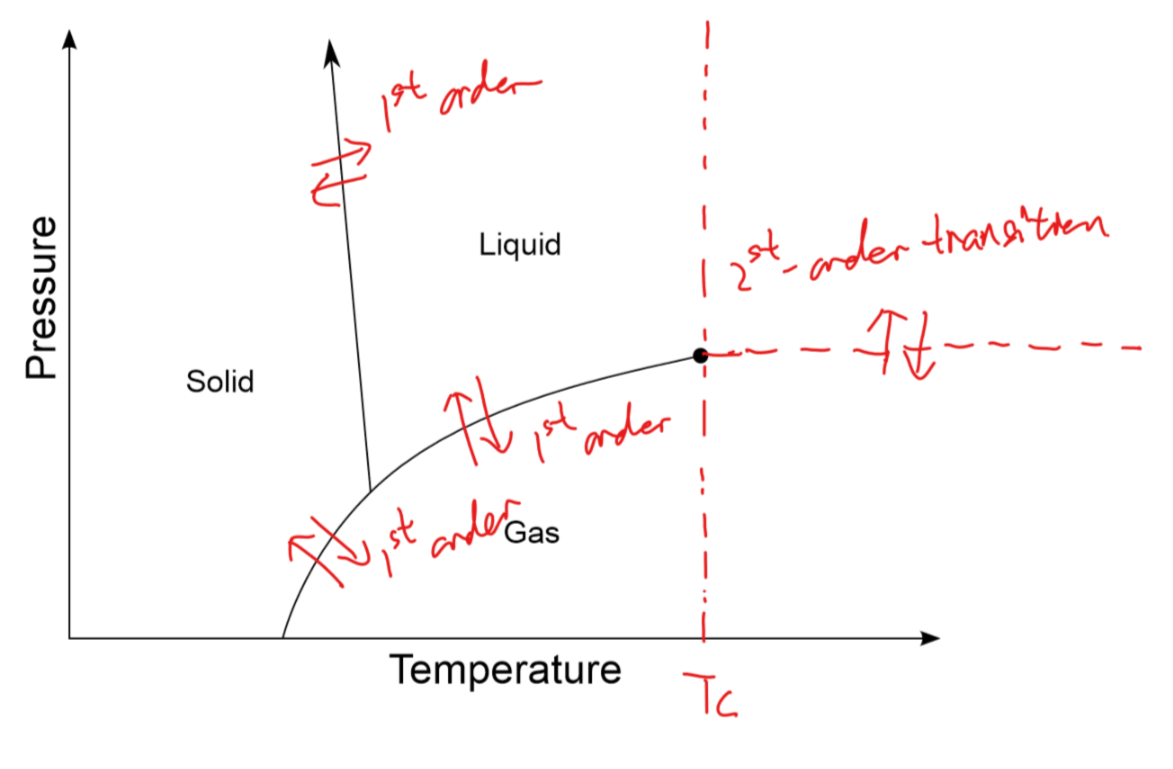
\includegraphics[scale=0.5]{PIC/hw1.png}
	\end{figure}
\end{exer}
\begin{exer}
	By the homogeneous relation
\[
f(t,h)= b^{-d}f(b^{y_t} t, b^{y_h} h)
\]
we have 
\[
f(t,h)= t^{\frac{d}{y_t}}g(\alpha)
\]
where $g(\alpha) = f(1,\alpha)$ and $\alpha = t^{-\frac{y_h}{y_t}}h$. It is easy to see that $\alpha$ is invariance under scaling transformation $x \to x/b$.
Hence we have 
\[
\begin{aligned}
&C(t,0) = -T \frac{\partial ^2 f}{\partial T ^2}\big|_{h=0} = - \frac{1}{T_c} t^{\frac{d}{y_t}-2}g''(0) \\
& M(t,0) = -\frac{\partial f}{\partial B}\big|_{h=0} =t^{\frac{d-y_h}{y_t}}g'(0)\\
& \chi(t,0) = \frac{\partial^2 f}{\partial B^2}\big|_{h=0} = t^{(d-2y_h)/y_t} g''(0)\\
\end{aligned}
\]
As function with single variable $h$, $\lim_{t \to 0}  M(t,h) \sim h^{\frac{1}{\delta}}$, which implies that $g'(\alpha) \sim \alpha^{\frac{1}{\delta}}$ since $\alpha$ is linear function of $h$. Hence we have 
\[
\lim_{t \to 0} M = \lim_{t \to 0} t^{(d-y_n - \frac{y_n}{\delta})}h ^{1/\delta}
\]
since it is non-zero, we have $d- y_n - y_n \frac{1}{\delta}=0$. Hence we have 
\[
\delta = \frac{y_h}{d-y_h}
\]	
\end{exer}
\begin{exer}
	We have following relation
	\begin{equation}\label{eq1}
	G_{\sigma}(\mathbf{r};t,h) = t^{-2x_{\sigma}}G_\sigma (\frac{\mathbf{r}}{b};b^{y_t}t,b^{y_h}h)
	\end{equation}
	Let $h=0, K= b^{y_t}t$,	
	\[
	G_{\sigma}(\mathbf{r};t,0) = t^{2x_{\sigma}/y_{t}}G_\sigma (\frac{\mathbf{r}}{K t^{-1/y_{t}}};K,0)
	\]
	Since $ G_{\sigma}(\mathbf{r}) \sim r^{-\tau} e^{-\frac{r}{\xi}}$, we have $\xi \sim t^{-1/y_t}$. It implies $\nu = 1/y_t$. With relation \ref{eq1}, we have 
	\[
	\chi(t,h)= \frac{1}{T} \int d^d \mathbf{r} G_\sigma (\mathbf{r};t,h)= t^{d-2x_\sigma} \chi (b^{y_t}t, b^{y_h}h)
	\]
	So $\gamma = (d-2x_\sigma)/y_t$. But we have $\eta = 2 x_\sigma +2 -d$ for finite limit of $G(r)$ when $t \to 0$ and $h=0$. Therefore, we get
	\[
	\gamma = \nu(2-\eta)
	\]With scaling relations
	\[
	\begin{aligned}
	\alpha + 2 \beta + \gamma =2\\
	\alpha + \beta (1+\delta) =2\\
	\end{aligned}
	\]
	and $\alpha = 2 -d \nu$, we have
	\[
	\begin{aligned}
	\beta &= \frac{d\nu -2\nu + \nu \eta}{2}\\
	\delta &= \frac{d-\eta +2}{d+\eta -2}\\
	\end{aligned}
	\]
	\end{exer}
\begin{exer}
	By listed commutation relations, we have, for $r, s > 0$,
	\[
	\begin{aligned}
	&[D, J_{rs}]= [D, L_{rs}] = \frac{i}{2} [D, [K_r, P_s]]\\
	 & =-\frac{i}{2}\big([P_s,[D,K_r]]+ [K_r,[P_s,D]]\big)\\
	 & =\frac{1}{2}[P_s, K_r] -\frac{1}{2}[K_r, P_s]\\
	 &=0
	\end{aligned}
	\]
	For $r=-1,s=0$, $[D,J_{rs}]= [D,D]=0$. For $r=-1, s\neq 0$, $[D,J_{-1,s}]=[D,\frac{1}{2}(P_s - K_s)]= \frac{i}{2}(P_s +K_s)$. For $r=0$, $[D, J_{0s}] = \frac{i}{2}(P_s - K_s)$. Hence (2,25) is satisfied when $(m,n)=(-1,0)$.
	
	If $(m,n)=(-1,n)$, then we have 
	\[
	[J_{mn},J_{rs}] = \frac{1}{2}[P_n, J_{rs}] -\frac{1	}{2} [K_n, J_{rs}]
	\]
	With listed commutation relations, we can easily check it coincides with (2,25) respectively. Similarly check in the case of $(m,n)= (0,n)$. 
\end{exer}
\end{document}